% =============================================================================
% 10-virtual-memory-storage-notes.tex -- Lecture Notes for Week 10
% DERIVED ARTIFACT. Source of truth: Slides/CS401/10-virtual-memory-storage.tex.
% The Notes reorganize the deck by topic while preserving its content, notation,
% diagrams, worked examples, and citations.
%
% Anchor reading:
%   * Stallings, 11e: CAM in Sec. 5.2 (PDF pp. 193--194); external memory
%     Secs. 7.1--7.4 (PDF pp. 265--292); memory management Sec. 9.3
%     (PDF pp. 376--389). Page citations below follow the indexed PDF.
%   * Patterson & Hennessy, ARM 5e: virtual memory Sec. 5.7 (p. 441) and
%     RAID Sec. 5.11 (p. 481).
%   * Hamacher Ch. 8 remains a chapter-level syllabus anchor only.
%
% Compile from Notes/CS401 on Windows/MiKTeX:
%   TEXINPUTS="../../Preambles;" xelatex -interaction=nonstopmode 10-virtual-memory-storage-notes.tex
%   BIBINPUTS="../..;" bibtex 10-virtual-memory-storage-notes
%   TEXINPUTS="../../Preambles;" xelatex -interaction=nonstopmode 10-virtual-memory-storage-notes.tex
%   TEXINPUTS="../../Preambles;" xelatex -interaction=nonstopmode 10-virtual-memory-storage-notes.tex
% =============================================================================

\documentclass[11pt]{article}
\usepackage[margin=1in]{geometry}
\usepackage{array}
% =============================================================================
% Preambles/header.tex — shared LaTeX/Beamer preamble for this project
%
% Use from a Beamer lecture by prepending:
%     \input{header}
% and compiling with TEXINPUTS=../Preambles:$TEXINPUTS (the /compile-latex
% skill does this automatically).
%
% PALETTE CONTRACT. Color names defined here MUST match the names in
% Quarto/theme-template.scss so Beamer and Quarto renderings use the same
% palette. The scripts/check-palette-sync.sh script enforces this.
%
% To customize: edit the HEX values below AND the matching $variable in
% Quarto/theme-template.scss, then run scripts/check-palette-sync.sh.
% =============================================================================

% -----------------------------------------------------------------------------
% Engine detection + encoding
%
% Our /compile-latex skill uses XeLaTeX, where inputenc is unnecessary and
% can produce encoding warnings. Only load inputenc under pdfTeX.
% -----------------------------------------------------------------------------
\usepackage{iftex}
\ifPDFTeX
  \usepackage[utf8]{inputenc}
\fi

\usepackage{amsmath, amssymb, amsthm}
\usepackage{booktabs}
\usepackage{graphicx}

% -----------------------------------------------------------------------------
% PALETTE — mirrors Quarto/theme-template.scss variable names.
% Load xcolor and define colors BEFORE anything that references them
% (notably hyperref, hypersetup, and the Beamer color assignments).
% -----------------------------------------------------------------------------
\usepackage{xcolor}

\definecolor{primary-blue}{HTML}{012169}      % headings, accents
\definecolor{primary-gold}{HTML}{B9975B}      % emphasis, borders
\definecolor{highlight-yellow}{HTML}{F2A900}  % markers, alerts
\definecolor{light-bg}{HTML}{E8EDF5}          % title / section backgrounds
\definecolor{jet}{HTML}{1A1A1A}               % body text

% Semantic colors (used in diagrams and annotations)
\definecolor{positive}{HTML}{15803D}          % good / observed / identified
\definecolor{negative}{HTML}{B91C1C}          % bad / problematic / bias
\definecolor{neutral}{HTML}{525252}           % reference / context

% Highlight accents (match .hi-* classes in the SCSS)
\definecolor{hi-slate}{HTML}{314F4F}
\definecolor{hi-green}{HTML}{2E8B57}
\definecolor{hi-red}{HTML}{C41E3A}

% Semantic aliases so skill templates and snippets can write
% \textcolor{accent}{...} without hard-coding "primary-blue".
\colorlet{accent}{primary-blue}
\colorlet{accent2}{primary-gold}

% -----------------------------------------------------------------------------
% Hyperref — loaded AFTER xcolor + palette so link colors resolve.
% -----------------------------------------------------------------------------
\usepackage{hyperref}
\hypersetup{colorlinks=true, linkcolor=primary-blue, urlcolor=primary-blue,
            citecolor=primary-blue, pdfborder={0 0 0}}

% -----------------------------------------------------------------------------
% Course code — set once per deck (after \input{header}, before \begin{document})
% via \coursecode{CS401}. Shown in the footer on every slide so a deck's course
% is identifiable without opening the title page. Empty by default.
% -----------------------------------------------------------------------------
\makeatletter
\newcommand{\coursecode}[1]{\gdef\@coursecodetext{#1}}
\gdef\@coursecodetext{}
\makeatother

% -----------------------------------------------------------------------------
% Beamer theme assignments (only apply under Beamer).
%
% We detect Beamer via \@ifclassloaded{beamer}, which is the documented,
% non-internal way. This must be wrapped in \makeatletter/\makeatother
% because \@ifclassloaded contains an @-catcode character.
% -----------------------------------------------------------------------------
\makeatletter
\@ifclassloaded{beamer}{%
  \usefonttheme{professionalfonts}
  \setbeamercolor{structure}{fg=primary-blue}
  \setbeamercolor{frametitle}{fg=primary-blue}
  \setbeamercolor{title}{fg=primary-blue}
  \setbeamercolor{subtitle}{fg=primary-gold}
  \setbeamercolor{author}{fg=primary-blue}
  \setbeamercolor{institute}{fg=neutral}
  \setbeamercolor{date}{fg=primary-gold}
  \setbeamercolor{itemize item}{fg=primary-blue}
  \setbeamercolor{itemize subitem}{fg=primary-gold}
  \setbeamercolor{alerted text}{fg=primary-gold}
  \setbeamercolor{block title}{fg=white, bg=primary-blue}
  \setbeamercolor{block body}{bg=light-bg}
  % Semantic block variants: block=definition/concept (blue), exampleblock=
  % worked example (green/positive), alertblock=key takeaway or caution (gold).
  % Keep to <=2 colored boxes per slide across ALL three variants (INV-7).
  \setbeamercolor{block title example}{fg=white, bg=positive}
  \setbeamercolor{block body example}{bg=light-bg}
  \setbeamercolor{block title alerted}{fg=white, bg=primary-gold}
  \setbeamercolor{block body alerted}{bg=light-bg}

  % Minimal footer: course code (left) + page X / N (right), no navigation clutter
  \setbeamertemplate{navigation symbols}{}
  \setbeamertemplate{footline}{%
    \color{neutral}\footnotesize\hspace{0.7em}\@coursecodetext\hfill
    \insertframenumber/\inserttotalframenumber\hspace{0.7em}\vspace{0.3em}}
}{}
\makeatother

% -----------------------------------------------------------------------------
% TikZ setup — libraries the snippet gallery uses
% -----------------------------------------------------------------------------
\usepackage{tikz}
\usetikzlibrary{arrows.meta, positioning, calc, decorations.pathreplacing,
                fit, shapes.geometric, backgrounds}

% Shared TikZ styles — snippets and hand-written diagrams can pick these up
% via `\begin{tikzpicture}[every node/.style={...}]` or by naming specific
% styles (e.g., `\node[dag-node] (X) at (0,0) {X};`).
\tikzset{
  % Node styles for causal DAGs and similar
  dag-node/.style = {
    draw=primary-blue, fill=light-bg, rounded corners=2pt,
    minimum width=1.2cm, minimum height=0.9cm, align=center, font=\small
  },
  decision-node/.style = {
    draw=primary-gold, fill=white, diamond, aspect=1.8,
    minimum width=1.8cm, minimum height=1.2cm, align=center, font=\small,
    inner sep=1pt
  },
  % Edge styles — observed vs counterfactual
  observed-edge/.style = {-{Latex[length=2.5mm]}, thick, draw=jet},
  counterfactual-edge/.style = {-{Latex[length=2.5mm]}, thick, draw=neutral, dashed},
  confound-edge/.style = {-{Latex[length=2.5mm]}, thick, draw=negative, dashed},
  % Data-point styles for plots
  observed-dot/.style = {fill=primary-blue, draw=primary-blue, circle, inner sep=1.2pt},
  counterfactual-dot/.style = {fill=white, draw=neutral, circle, inner sep=1.2pt}
}

% -----------------------------------------------------------------------------
% Convenience macros
% -----------------------------------------------------------------------------
\newcommand{\muted}[1]{\textcolor{neutral}{#1}}
\newcommand{\key}[1]{\textcolor{primary-gold}{\textbf{#1}}}
\newcommand{\good}[1]{\textcolor{positive}{#1}}
\newcommand{\bad}[1]{\textcolor{negative}{#1}}

% Standout frame macro: full-bleed dark background for section transitions.
% Beamer-only (uses \begin{frame}/\setbeamercolor/\usebeamerfont) -- do not
% call from an article-class file (e.g. Notes/<CODE>/*-notes.tex). \muted,
% \key, \good, \bad, and \coursecode above are plain xcolor/gdef and are
% safe to use from either class; verified when Notes/article-class support
% was added.
% Expand: \transitionslide{Your transition title}
\newcommand{\transitionslide}[1]{%
  \begingroup
  \setbeamercolor{background canvas}{bg=primary-blue}
  \begin{frame}[plain]
    \centering
    \vfill
    {\usebeamerfont{title}\color{white}\Large #1\par}
    \vfill
  \end{frame}
  \endgroup
}

% Section divider frame (Beamer-only), an alternative to \transitionslide with a
% darker two-line style: near-black (jet) background, a small white label line
% above a larger gold title, and a thin gold rule along the bottom edge.
% Expand: \sectiondivider{Section 2}{Pointers}
\newcommand{\sectiondivider}[2]{%
  \begingroup
  \setbeamercolor{background canvas}{bg=jet}
  \begin{frame}[plain]
    \vspace*{3.0cm}
    {\color{white}\ttfamily\large #1\par}
    \vspace{0.5cm}
    {\color{primary-gold}\LARGE #2\par}
    \begin{tikzpicture}[remember picture, overlay]
      \draw[primary-gold, line width=2.5pt]
        ($(current page.south west)+(0,0.1)$) -- ($(current page.south east)+(0,0.1)$);
    \end{tikzpicture}
  \end{frame}
  \endgroup
}

% -----------------------------------------------------------------------------
% Channel watermark — "Concepts That Click" (YouTube).
%
% Article-class files (CompetitiveExam Q/A sets, Notes, Assignments) get a
% light diagonal draft watermark on every page plus a centered footer naming
% the channel. Beamer decks get a subtle TikZ background watermark instead
% (the footline already carries the course code). Centralized here so every
% MCQ PDF is branded without per-file edits.
% -----------------------------------------------------------------------------
\makeatletter
\@ifclassloaded{article}{%
  \usepackage{draftwatermark}
  \SetWatermarkText{Concepts That Click}
  \SetWatermarkScale{1}
  \SetWatermarkFontSize{2cm}
  \SetWatermarkLightness{0.86}
  \SetWatermarkAngle{45}
  \usepackage{fancyhdr}
  \pagestyle{fancy}
  \fancyhf{}
  \fancyfoot[C]{\footnotesize\textcolor{neutral}{Concepts That Click~|~YouTube: \href{https://www.youtube.com/@concepts.thatclick}{@concepts.thatclick}}}
  \renewcommand{\headrulewidth}{0pt}
  \renewcommand{\footrulewidth}{0pt}
  \fancypagestyle{plain}{%
    \fancyhf{}%
    \fancyfoot[C]{\footnotesize\textcolor{neutral}{Concepts That Click~|~YouTube: \href{https://www.youtube.com/@concepts.thatclick}{@concepts.thatclick}}}%
    \renewcommand{\headrulewidth}{0pt}%
    \renewcommand{\footrulewidth}{0pt}%
  }
}{}
\@ifclassloaded{beamer}{%
  \setbeamertemplate{background}{%
    \begin{tikzpicture}[remember picture, overlay]
      \node[rotate=45, opacity=0.055, align=center]
        at (current page.center)
        {\Huge\textcolor{neutral}{Concepts That Click}};
    \end{tikzpicture}%
  }
}{}
\makeatother 
\coursecode{CS401}

\renewcommand{\thesection}{10.\arabic{section}}
\renewcommand{\thefigure}{10.\arabic{figure}}
\newtheorem{example}{Example}[section]

\newenvironment{definitionbox}[1]{%
  \par\noindent\textbf{Definition (#1).}\ \itshape
}{\par\vspace{0.3em}}

\usepackage{caption}

\title{Virtual Memory and Secondary Storage\\\large Lecture Notes --- Week 10}
\author{PCC CS-401: Computer Organization and Architecture}
\date{\today}

\begin{document}
\maketitle

\section{The Hierarchy Continues: From Cache to Storage}
\label{sec:intro}

Week 9 placed a small, fast cache between the CPU and a larger, slower main
memory. A cache line is found by mapping an address and checking a tag; a miss
fetches a block and may trigger replacement. The design goal was not to make
all memory fast, but to make the common case fast by exploiting locality.

This week asks whether the same idea can operate one level lower. If a
program's address space is larger than physical main memory, can a small,
fast level (DRAM) stand in for a larger, slower level (secondary storage)? The
answer requires six connected ideas:
\begin{enumerate}
  \item content-addressable lookup through associative memory and CAM;
  \item virtual addresses, page tables, and TLB translation;
  \item page faults and demand paging when a page is not resident;
  \item segmentation, partitioning, fragmentation, and allocation policies;
  \item HDDs, optical media, SSDs, and RAID as storage technologies; and
  \item a decision procedure that connects lookup, placement, failure
        response, and cost across Unit III.
\end{enumerate}

The running system has a 16-bit virtual address, 256-byte pages, and 8
physical frames. We first translate virtual address \texttt{0x2F34}, then
follow the page-fault and storage consequences of that translation.

\section{Associative Lookup and CAM}
\label{sec:associative}

\subsection{When Content Is the Lookup Key}

The cache question from Week 9 was: ``Is the block with this tag present?''
Under fully associative mapping, the tag may be in any cache line, so checking
one predetermined address is insufficient. A conventional RAM performs
\key{address $\to$ contents}; an associative lookup performs
\key{content pattern $\to$ matching row} by comparing a search key against
many stored entries in parallel. This is the standard CAM hardware treatment
of associative cache lookup (see Stallings, 11e, \S5.2, PDF pp.~193--194
\cite[\S5.2, PDF pp.~193--194]{Stallings2015_computer_organization}).

\begin{definitionbox}{Associative memory}
Associative memory is memory searched by the content pattern being sought,
rather than by one fixed address. Parallel comparison makes placement
flexible, but requires multiple comparators, match-selection logic, wiring,
area, energy, and verification effort.
\end{definitionbox}

\subsection{A CAM Lookup}

Content-addressable memory (CAM) compares the search key with every stored row
at once. The match vector identifies the row whose contents equal the key;
the row's associated data can then be read. In a TLB, the compared content is
typically a virtual page number together with address-space information, and
the matching entry supplies a physical frame number.

\begin{figure}[h]
  \centering
  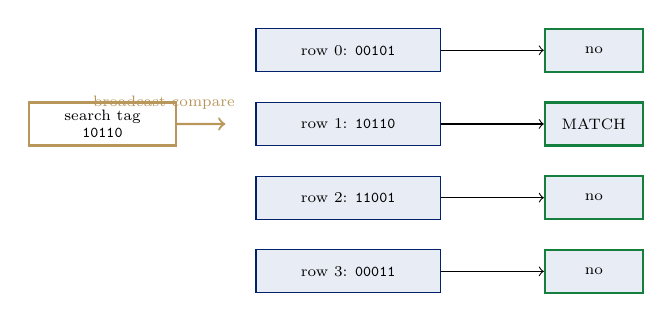
\begin{tikzpicture}[scale=0.78, transform shape,
      every node/.style={font=\scriptsize}]
    \node[draw=primary-gold, thick, fill=white, minimum width=2.4cm,
          minimum height=0.7cm, align=center] (KEY) at (0,2.4)
          {search tag\\\texttt{10110}};
    \node[draw=primary-blue, fill=light-bg, minimum width=3.0cm,
          minimum height=0.7cm, align=center] (R0) at (4.0,3.6)
          {row 0: \texttt{00101}};
    \node[draw=primary-blue, fill=light-bg, minimum width=3.0cm,
          minimum height=0.7cm, align=center] (R1) at (4.0,2.4)
          {row 1: \texttt{10110}};
    \node[draw=primary-blue, fill=light-bg, minimum width=3.0cm,
          minimum height=0.7cm, align=center] (R2) at (4.0,1.2)
          {row 2: \texttt{11001}};
    \node[draw=primary-blue, fill=light-bg, minimum width=3.0cm,
          minimum height=0.7cm, align=center] (R3) at (4.0,0.0)
          {row 3: \texttt{00011}};
    \node[draw=positive, thick, fill=light-bg, minimum width=1.6cm,
          minimum height=0.7cm, align=center] (M0) at (8.0,3.6) {no};
    \node[draw=positive, thick, fill=light-bg, minimum width=1.6cm,
          minimum height=0.7cm, align=center] (M1) at (8.0,2.4) {MATCH};
    \node[draw=positive, thick, fill=light-bg, minimum width=1.6cm,
          minimum height=0.7cm, align=center] (M2) at (8.0,1.2) {no};
    \node[draw=positive, thick, fill=light-bg, minimum width=1.6cm,
          minimum height=0.7cm, align=center] (M3) at (8.0,0.0) {no};
    \draw[->, thick, primary-gold] (KEY.east) -- (2.0,2.4);
    \node[primary-gold] at (1.0,2.75) {broadcast compare};
    \draw[->] (R0.east) -- (M0.west);
    \draw[->] (R1.east) -- (M1.west);
    \draw[->] (R2.east) -- (M2.west);
    \draw[->] (R3.east) -- (M3.west);
  \end{tikzpicture}
  \caption{CAM compares one search tag with all rows in parallel and emits a
  match vector.}
  \label{fig:cam}
\end{figure}

The benefit is flexible placement: a key need not be assigned to one
predetermined row, reducing conflict misses. The cost is that all comparisons
and the match-selection logic operate in parallel. This is the same
placement-versus-hardware trade-off behind fully associative caches and TLBs.
Associative does not mean ``random''; it describes the lookup method.

\section{Virtual Memory, Paging, and Address Translation}
\label{sec:paging}

\subsection{A Private Address Space Backed by DRAM and Storage}

A process should be able to use a simple, contiguous address space without
knowing which physical locations are free or which other process owns them. A
\key{virtual address} is generated by the CPU for the process. The
memory-management unit (MMU) translates it to a \key{physical address} in
main memory. Pages are the virtual-memory analogue of cache blocks, and
physical frames are the fixed-size slots that hold them. If the page is absent,
the hardware raises a \key{page fault}; the operating system can fetch the
page from secondary storage (Patterson and Hennessy, ARM 5e, \S5.7, p.~441
\cite[\S5.7, p.~441]{PattersonHennessy2017_computer_organization_design}).

\begin{definitionbox}{Paging}
Paging divides a virtual address space into fixed-size pages and physical
memory into equal-size frames. Translation replaces the virtual page number
with a physical frame number while preserving the offset within the page.
\end{definitionbox}

\subsection{The Address Fields}

For the running system, the virtual address width is $V=16$ bits and the page
size is $256=2^8$ bytes. Physical memory has 8 frames, or $2^3$ frames.
Therefore:
\begin{itemize}
  \item the virtual address space has $2^{16}=65{,}536$ bytes $=64$~KiB;
  \item the number of virtual pages is $2^{16}/2^8=2^8=256$;
  \item physical memory has $8\times256=2{,}048$ bytes $=2$~KiB;
  \item a virtual address contains an 8-bit virtual page number (VPN) and an
        8-bit page offset; and
  \item a physical address contains a 3-bit physical frame number (PFN) and
        the same 8-bit offset.
\end{itemize}

The key invariant is that translation changes only the page/frame field. The
offset within a page is never changed.

\begin{figure}[h]
  \centering
  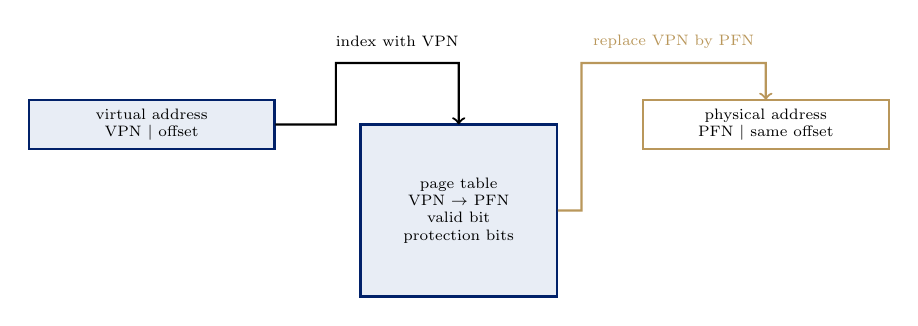
\begin{tikzpicture}[scale=0.78, transform shape,
      every node/.style={font=\scriptsize}]
    \node[draw=primary-blue, thick, fill=light-bg, minimum width=4.0cm,
          minimum height=0.8cm, align=center] (VA) at (0,3.4)
          {virtual address\\VPN \textbar\ offset};
    \node[draw=primary-blue, thick, fill=light-bg, minimum width=3.2cm,
          minimum height=2.8cm, text width=2.8cm, align=center] (PT) at (5.0,2.0)
          {page table\\VPN $\to$ PFN\\valid bit\\protection bits};
    \node[draw=primary-gold, thick, fill=white, minimum width=4.0cm,
          minimum height=0.8cm, align=center] (PA) at (10.0,3.4)
          {physical address\\PFN \textbar\ same offset};
    \draw[->, thick] (VA.east) -- (3.0,3.4) -- (3.0,4.4) --
          (5.0,4.4) -- (5.0,3.4);
    \node at (4.0,4.75) {index with VPN};
    \draw[->, thick, primary-gold] (PT.east) -- (7.0,2.0) -- (7.0,4.4) --
          (10.0,4.4) -- (10.0,3.8);
    \node[primary-gold] at (8.5,4.75) {replace VPN by PFN};
  \end{tikzpicture}
  \caption{Paging translation indexes the page table with the VPN, replaces
  the VPN by a PFN, and preserves the page offset.}
  \label{fig:paging}
\end{figure}

The page table records the current physical frame, validity, and access
permissions for each virtual page. A valid entry gives a resident mapping; an
invalid entry signals that the operating system must intervene.

\begin{example}[Translating \texttt{0x2F34}]
\label{ex:translation}
First write the virtual address in binary:
\[
  \texttt{0x2F34}=0010\,1111\,0011\,0100_2.
\]
The eight high bits are the VPN and the eight low bits are the offset:
\[
  \underbrace{0010\,1111}_{\mathrm{VPN}=\texttt{0x2F}=47}\quad
  \underbrace{0011\,0100}_{\mathrm{offset}=\texttt{0x34}=52}.
\]
Suppose the page-table entry for VPN 47 is valid and maps it to physical frame
5, whose three-bit representation is $101_2$. The physical address is
\[
  5\times256+52=1{,}332\text{ bytes}.
\]
Equivalently, concatenate the frame field and the unchanged offset:
\[
  \texttt{0x5}\,||\,\texttt{0x34}=\texttt{0x534}.
\]
The low eight bits stayed \texttt{0x34}; only the page number changed.
\end{example}

\subsection{The TLB: A Cache of Translations}

\begin{definitionbox}{Translation Lookaside Buffer}
A TLB is a small associative cache of recent page-table mappings, from VPN to
PFN. It is checked before the larger page table (Patterson and Hennessy, ARM
5e, \S5.7, p.~441 \cite[\S5.7, p.~441]{PattersonHennessy2017_computer_organization_design}).
\end{definitionbox}

The translation path is:
\begin{enumerate}
  \item split the CPU's virtual address into VPN and offset;
  \item compare the VPN with stored TLB entries in parallel;
  \item on a TLB hit, obtain the PFN, concatenate it with the offset, and
        access DRAM; or
  \item on a TLB miss, consult the page table. If its entry is valid, fill the
        TLB and retry; if it is invalid, take a page fault.
\end{enumerate}
The TLB is associative because the desired VPN may occupy any TLB entry; its
match is a content lookup rather than an indexed lookup at one fixed location.

\section{Page Faults, Segmentation, and Allocation}
\label{sec:management}

\subsection{Demand Paging}

\begin{definitionbox}{Page fault}
A page fault occurs when translation identifies a virtual page that is not
currently resident in a physical frame. It is not automatically a program
error: the operating system may make the reference legal by loading the page
from storage.
\end{definitionbox}

The fault-handling sequence is explicit:
\begin{enumerate}
  \item hardware traps to the operating-system page-fault handler;
  \item the handler checks the access. An illegal address or permission
        failure terminates the process, while a legal nonresident page is
        located in storage;
  \item if no free frame exists, the system chooses a victim page, writes it
        back if it is dirty, and reads the requested page into that frame;
  \item the page table and TLB are updated, the requested page is marked valid,
        and the faulting instruction is restarted.
\end{enumerate}

This is \key{demand paging}: storage is a backing level, not a substitute for
DRAM's latency. The memory-management treatment is indexed in Stallings,
11e, \S9.3, PDF pp.~376--389.

\subsection{Why Page Size Is a Trade-off}

Large pages reduce the number of page-table entries and can transfer data
efficiently when spatial locality is strong. They also waste more space when
only a small part of a page is used and transfer more irrelevant data on a
fault. Small pages reduce internal waste and provide finer protection, but
require larger page tables and create more translation overhead. A useful page
size balances page-table cost, transfer cost, fragmentation, and the program's
locality.

\subsection{Segmentation}

\begin{definitionbox}{Segmentation}
Segmentation represents an address space as variable-sized logical regions,
such as code, data, stack, or a shared library. A logical address consists of
a segment number and an offset.
\end{definitionbox}

A segment-table entry supplies a base address, a limit, and access permissions.
Translation first checks
\[
  0\leq\text{offset}<\text{limit},
\]
then forms
\[
  \text{physical address}=\text{base}+\text{offset}.
\]
Protection and sharing can follow program structure: code can be read/execute,
while data can be read/write. The variable sizes make external fragmentation
possible; paging avoids external fragmentation by using fixed-size frames.
Stallings treats segmentation as part of memory management in \S9.3, PDF
pp.~376--389; Hamacher Ch.~8 is the syllabus-level anchor for the same
standard treatment.

\begin{center}
\footnotesize
\begin{tabular}{@{}>{\raggedright\arraybackslash}p{2.2cm}>{\raggedright\arraybackslash}p{3.6cm}>{\raggedright\arraybackslash}p{3.6cm}>{\raggedright\arraybackslash}p{2.8cm}@{}}
\toprule
\textbf{Scheme} & \textbf{Allocation unit} & \textbf{Strength} & \textbf{Main cost} \\
\midrule
Paging & Fixed-size page/frame & Simple placement; no external fragmentation; easy swapping & Internal fragmentation; page-table/TLB overhead \\
Segmentation & Variable-size logical segment & Natural protection/sharing; programmer-visible units & External fragmentation; compaction or complex allocation \\
Paged segmentation & Segments divided into pages & Combines logical protection with fixed-size placement & Two-level translation and more metadata \\
\bottomrule
\end{tabular}
\end{center}

The exam habit is to state the unit first. Fixed-size units imply pages,
frames, and internal fragmentation. Variable-size units imply segments,
holes, and external fragmentation.

\subsection{Contiguous Allocation and Hole Selection}

Suppose free memory contains holes of $100$, $500$, $200$, $300$, and
$600$~KiB, and a process requests $212$~KiB. The three policies choose
different holes:
\begin{itemize}
  \item \key{First fit} chooses the first adequate hole, $500$~KiB, leaving
        $500-212=288$~KiB.
  \item \key{Best fit} chooses the smallest adequate hole, $300$~KiB, leaving
        $300-212=88$~KiB, but may create many tiny holes.
  \item \key{Worst fit} chooses the largest hole, $600$~KiB, leaving
        $600-212=388$~KiB and preserving medium-sized holes elsewhere.
\end{itemize}
In every case, the selected hole is split into the allocated block and a
smaller free hole.

\begin{example}[Comparing the three policies]
\label{ex:allocation}
For the hole list $(100,500,200,300,600)$~KiB and request $212$~KiB, the
post-placement free lists are:
\begin{itemize}
  \item first fit: $(100,288,200,300,600)$~KiB;
  \item best fit: $(100,500,200,88,600)$~KiB; and
  \item worst fit: $(100,500,200,300,388)$~KiB.
\end{itemize}
The policy choice is therefore a choice about the shape of future holes, not
just about where this one process is placed.
\end{example}

\subsection{Fragmentation and Policy Choice}

\begin{definitionbox}{Internal and external fragmentation}
\textbf{Internal fragmentation} is unused space inside an allocated
fixed-size unit, such as the unused tail of a page or frame. \textbf{External
fragmentation} occurs when enough total free space exists, but it is divided
into non-contiguous holes and cannot satisfy one contiguous request.
\end{definitionbox}

Paging largely removes external fragmentation because any free frame can hold
any page, but it does not remove internal fragmentation: the last page of a
process is often only partly occupied. Segmentation matches logical units well,
but allocation must manage holes; compaction moves allocated segments and is
expensive.

For a real-time allocator receiving many requests between 90 and 120~KiB,
first fit is a defensible default because it usually searches less. Best fit is
defensible only if measurements show that preserving larger holes is worth the
extra search and small-hole production. Worst fit is defensible only if the
workload benefits from retaining useful medium-sized holes. The engineering
answer names the workload and metric, rather than naming a policy in isolation.

\section{Secondary Storage}
\label{sec:storage}

\subsection{HDD Access and Geometry}

An HDD stores bits magnetically on rotating platters. A request selects a
surface and track, waits for the desired sector to rotate under the head, and
then transfers the data. Its access time is decomposed as
\[
  T_{access}=T_{seek}+T_{rotation}+T_{transfer}+T_{controller}.
\]
\textbf{Seek time} moves the actuator to the target track. \textbf{Rotational
latency} waits for the target sector; average latency is approximately half a
rotation. \textbf{Transfer time} reads or writes the sector once positioned.
Stallings treats these components in \S7.1, PDF p.~265. Sequential access
amortizes seek and rotation, whereas random page faults can be dominated by
positioning time.

\begin{figure}[h]
  \centering
  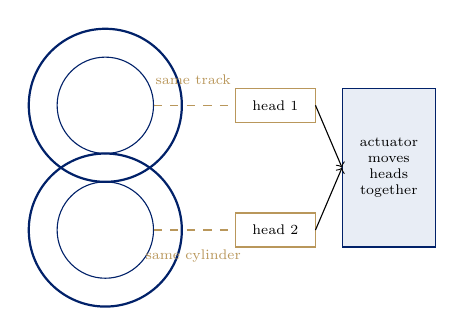
\begin{tikzpicture}[scale=0.72, transform shape,
      every node/.style={font=\scriptsize}]
    \draw[draw=primary-blue, thick] (2.0,2.2) circle (1.35);
    \draw[draw=primary-blue] (2.0,2.2) circle (0.85);
    \draw[draw=primary-blue, thick] (2.0,0.0) circle (1.35);
    \draw[draw=primary-blue] (2.0,0.0) circle (0.85);
    \node[draw=primary-gold, fill=white, minimum width=1.4cm,
          minimum height=0.6cm, align=center] (H1) at (5.0,2.2) {head 1};
    \node[draw=primary-gold, fill=white, minimum width=1.4cm,
          minimum height=0.6cm, align=center] (H2) at (5.0,0.0) {head 2};
    \node[draw=primary-blue, fill=light-bg, minimum width=1.6cm,
          minimum height=2.8cm, text width=1.4cm, align=center] (ACT) at
          (7.0,1.1) {actuator\\moves heads together};
    \draw[dashed, primary-gold] (2.85,2.2) -- (4.3,2.2);
    \draw[dashed, primary-gold] (2.85,0.0) -- (4.3,0.0);
    \node[primary-gold] at (3.55,2.65) {same track};
    \node[primary-gold] at (3.55,-0.45) {same cylinder};
    \draw[->] (H1.east) -- (ACT.west);
    \draw[->] (H2.east) -- (ACT.west);
  \end{tikzpicture}
  \caption{HDD geometry: the actuator moves heads together, so corresponding
  tracks across platter surfaces form a cylinder.}
  \label{fig:hdd}
\end{figure}

A \textbf{cylinder} is the set of tracks at the same radius across surfaces.
Keeping related blocks nearby reduces movement and improves effective
throughput; this is storage-level spatial locality.

\subsection{RAID: Parallelism and Recovery}

\begin{definitionbox}{RAID}
RAID (Redundant Array of Independent Disks) combines multiple physical disks
and presents a logical storage system. Its design dimensions are striping for
parallelism, mirroring or parity for recovery, and the number of disks left
available after redundancy.
\end{definitionbox}

\begin{center}
\footnotesize
\begin{tabular}{@{}>{\raggedright\arraybackslash}p{1.0cm}>{\raggedright\arraybackslash}p{5.0cm}>{\raggedright\arraybackslash}p{5.0cm}@{}}
\toprule
\textbf{Level} & \textbf{Idea} & \textbf{Trade-off} \\
\midrule
RAID 0 & Block striping, no redundancy & High throughput; one disk failure loses the array \\
RAID 1 & Mirroring & Simple recovery; about half raw capacity \\
RAID 5 & Striping with distributed single parity & One-disk failure tolerance; parity-write cost \\
RAID 6 & Striping with distributed dual parity & Two-disk failure tolerance; more parity overhead \\
\bottomrule
\end{tabular}
\end{center}

RAID levels and their performance/reliability trade-offs are indexed in
Stallings, 11e, \S7.2, PDF pp.~276--288, and Patterson and Hennessy, ARM 5e,
\S5.11, p.~481.

\begin{example}[RAID 5 parity recovery]
\label{ex:raid}
Suppose corresponding bytes on three disks are
\[
  D_0=1010,\qquad D_1=0110,\qquad D_2=1100.
\]
RAID 5 stores the parity byte
\[
  P=D_0\oplus D_1\oplus D_2.
\]
First,
\[
  1010\oplus0110=1100,
  \qquad 1100\oplus1100=0000,
\]
so $P=0000$. If disk $D_1$ fails, XOR the surviving data and parity:
\[
  D_1=D_0\oplus D_2\oplus P
     =1010\oplus1100\oplus0000=0110.
\]
The missing block is recovered exactly. One failure is recoverable because
parity preserves the XOR relation; two simultaneous failures require more
independent parity, as in RAID 6.
\end{example}

\subsection{Optical Media and Workload Choice}

Optical media encode information in a spiral track of pits and lands. A laser
reads changing reflectivity and the drive converts that signal into bits.
Common capacities are approximately 700~MB for a CD, 4.7~GB for a
single-layer, single-sided DVD, and 25~GB for a single-layer Blu-ray. The
shorter-wavelength blue-violet laser and tighter track geometry allow Blu-ray
to store more data. Read-only, recordable, and rewritable variants differ in
how the recording layer changes. Optical media are removable and inexpensive
per disc, but slower and less convenient for frequent updates than SSDs. This
is standard secondary-storage treatment; Stallings indexes CD/DVD/Blu-ray in
\S7.4, PDF p.~292.

The medium should follow the bottleneck:
\begin{center}
\footnotesize
\begin{tabular}{@{}>{\raggedright\arraybackslash}p{2.3cm}>{\raggedright\arraybackslash}p{3.0cm}>{\raggedright\arraybackslash}p{3.0cm}>{\raggedright\arraybackslash}p{3.9cm}@{}}
\toprule
\textbf{Medium} & \textbf{Strength} & \textbf{Weakness} & \textbf{Good fit} \\
\midrule
HDD & Low cost per bit; large capacity & Mechanical seek and rotation & Bulk data, sequential files, cold storage \\
SSD/flash & Low latency; no moving head & Write/erase limits; higher cost per bit & OS/apps, random access, active working sets \\
Optical & Removable; useful for distribution/archive & Slow updates; lower capacity per medium & Media distribution and offline copies \\
RAID array & Parallelism plus optional redundancy & More controllers, disks, parity or mirror overhead & Servers needing throughput and availability \\
\bottomrule
\end{tabular}
\end{center}

The design question is whether the bottleneck is latency, throughput, capacity,
failure recovery, or cost. The answer follows from that bottleneck.

\section{Unit III Synthesis and Exam Procedure}
\label{sec:synthesis}

Across the hierarchy, the same four-part design pattern recurs:
\begin{enumerate}
  \item identify the \key{unit}: line, page, segment, block, or stripe;
  \item identify \key{lookup/placement}: tag comparison, page table/TLB,
        hole selection, disk geometry, or RAID mapping;
  \item state the \key{miss/failure response}: fetch a block, handle a page
        fault, split or compact a hole, seek and transfer, or reconstruct from
        redundancy; and
  \item state the \key{cost}: hardware, latency, capacity waste,
        fragmentation, bandwidth, or redundancy overhead.
\end{enumerate}

Week 9 made DRAM appear faster through cache. Week 10 makes storage-backed
capacity appear like a larger private memory through virtual memory, while
page faults expose the true cost. No level removes the cost; it changes when
and where the cost is paid.

When a program repeatedly touches a small set of pages but both its TLB miss
rate and page-fault rate are high, investigate four facts: TLB capacity and
associativity may be too small for the active VPNs; too few physical frames may
be causing repeated faults and thrashing; page size may be fetching irrelevant
data or creating excessive metadata; and an access pattern that alternates
across many pages may defeat replacement even when total memory seems large.

For an exam response, translate an address by splitting VPN and offset,
replacing only the VPN and preserving the offset. For a page fault, state the
trap, validity/protection check, victim selection, dirty write-back, page-in,
page-table/TLB update, and instruction restart. For paging versus segmentation,
name the unit and distinguish internal from external fragmentation. For an
allocation policy, show the hole list before and after placement. For an HDD,
decompose seek, rotational latency, transfer, and controller time. For RAID,
distinguish striping, mirroring, parity, capacity, throughput, and tolerated
failures. For associative memory, explain parallel comparison and its hardware
cost, then connect CAM/TLB lookup to fully associative cache mapping.

\subsection*{Exercises}
\begin{enumerate}
  \item A system has a 20-bit virtual address, 1~KiB pages, and 16 physical
        frames. Split virtual address \texttt{0xABCDE} into VPN and offset,
        and state the width of each physical-address field. Assume the VPN
        maps to frame 9 and compute the physical address.
  \item For holes of $(120, 280, 640, 200)$~KiB and a request of 190~KiB,
        show the resulting free list under first fit, best fit, and worst fit.
        Identify which policy leaves the smallest remainder in the selected
        hole.
  \item Given $D_0=1101$, $D_1=0011$, and $D_2=0101$, compute RAID 5 parity,
        then reconstruct $D_2$ after it fails.
  \item A workload alternates among more VPNs than the TLB can hold, while
        all referenced pages fit in physical memory. Diagnose why the TLB miss
        rate can be high while the page-fault rate remains low, and state one
        hardware fact and one access-pattern fact to investigate.
\end{enumerate}

\subsection*{Solutions}
\begingroup\small\raggedright
\begin{enumerate}
  \item A 1~KiB page has $2^{10}$ bytes, so the offset is 10 bits and the
        20-bit VPN is the high 10 bits. Since \texttt{0xABCDE} is
        $1010\,1011\,1100\,1101\,1110_2$, its low 10 bits are
      $00\,1101\,1110_2=\texttt{0x0DE}$ and its VPN is
        $1010\,1011\,11_2=687$. With 16 frames, the PFN is 4 bits. Mapping
        VPN 687 to frame 9 gives
      $9\times1024+\texttt{0x0DE}=9\times1024+222=9{,}438$,
      or \texttt{0x24DE}.
  \item First fit uses 280~KiB and leaves
        $(120,90,640,200)$~KiB. Best fit uses 200~KiB and leaves
        $(120,280,640,10)$~KiB. Worst fit uses 640~KiB and leaves
        $(120,280,450,200)$~KiB. Best fit leaves the smallest selected-hole
        remainder: 10~KiB.
  \item $P=1101\oplus0011\oplus0101$. Since
        $1101\oplus0011=1110$ and $1110\oplus0101=1011$, parity is
        $P=1011$. If $D_2$ fails, then
        $D_2=D_0\oplus D_1\oplus P=1101\oplus0011\oplus1011$.
        The first XOR is $1110$, and $1110\oplus1011=0101$, recovering the
        original block.
  \item The active translations can continually evict one another from a
        TLB whose capacity or associativity is too small, producing TLB misses
        even though every page-table entry is valid and resident. The hardware
        fact to investigate is TLB capacity/associativity; the access-pattern
        fact is whether the program cycles across more VPNs than the TLB can
        retain before reuse.
\end{enumerate}
\endgroup

\bibliographystyle{plain}
\bibliography{../../Bibliography_base}

\end{document}